\documentclass{article}
\usepackage{svg}
\usepackage[T1]{fontenc}
\usepackage[english]{babel}
\usepackage{hyphenat}
\usepackage{url}
\usepackage{graphicx}
\usepackage{subcaption}
\usepackage{listings}
\usepackage[utf8]{inputenc}
\usepackage[autostyle,english=american]{csquotes}
\usepackage{amsmath}
\usepackage{tikz}
\usepackage{float}
\usepackage{hyperref}
\usepackage[nohyperlinks]{acronym}
\usepackage[nonumberlist]{glossaries}
\usepackage{array}
\usepackage{tabularx}
\usepackage{amssymb}
\usepackage[style=ieee,autocite=footnote,giveninits=false,backend=biber]{biblatex}
% \usepackage{refcheck} % useful for checking and debugging
\usepackage{pdflscape}
\usepackage{pgfplots}
\usepackage{pgfplotstable}
\usepackage{csvsimple}
\usepackage{caption}
\usepackage{pdfpages}
\pgfplotsset{compat=1.18} % not sure whether this duplicates the versioning with the usepackage above; check if problems arise
\usepackage[english]{babel}
\usepackage{adjustbox}  % in the preamble
\usepackage{booktabs}
\usepackage[pass]{geometry} % keep template/default layout until margins are set after the title page
\usepackage{xcolor}
\usepackage{eurosym}
\usetikzlibrary{positioning,arrows.meta,fit,backgrounds,calc,shapes.geometric}
\addbibresource{Literatur.bib}
\newcolumntype{L}[1]{>{\raggedright\arraybackslash}p{#1}}
\makeglossaries

\newglossaryentry{retrofitting}
{
    name={retrofitting},
    description={the modification of an existing instrument, system or machine so that it gains functionality that was not part of the original design}
}

\newglossaryentry{backlash}
{
    name={backlash},
    description={lost motion that occurs when a drive mechanism changes direction before mechanical contact is re-established}
}

\newglossaryentry{frameanalysis}
{
    name={frame analysis},
    description={the reduced-rate image-processing path used for histogram computation, focus scoring, calibration support, and related live metrics}
}

\newglossaryentry{ometiff}
{
    name={OME-TIFF},
    description={an image format that stores microscopy image planes in TIFF files and encodes microscopy metadata using the OME data model}
}

\newglossaryentry{openloop}
{
    name={open-loop control},
    description={motion control in which motor commands are issued without continuous measurement of the resulting physical position}
}

\newglossaryentry{sangaboard}
{
    name={Sangaboard},
    description={an open-source motor-controller board that drives stepper motors and reports motor step counts to a host over a serial (UART) link}
}

\newglossaryentry{hysteresisband}
{
    name={hysteresis-band model},
    description={a backlash-compensation model that tracks a per-axis slack estimate within a band whose width equals the measured backlash, adding the slack take-up to a move only when the direction reverses}
}

\newglossaryentry{pixelscale}
{
    name={pixel scale},
    description={the physical distance in the specimen plane that corresponds to image pixels for a given objective and camera configuration, expressed in micrometers per pixel}
}

\newglossaryentry{stagescale}
{
    name={stage scale},
    description={the physical stage movement produced by one motor step, calibrated separately for the X and Y axes and expressed in micrometers per step}
}

\newglossaryentry{objectiveprofile}
{
    name={objective profile},
    description={the stored set of per-objective calibration values, including magnification, numerical aperture, pixel scale, backlash, depth-of-field steps, focus-stack step, and autofocus range}
}

\newglossaryentry{depthoffield}
{
    name={depth of field},
    description={the range of object distances along the optical axis that appears acceptably sharp at a given objective, used to choose focus-stack spacing and autofocus range}
}

\newglossaryentry{focusstacking}
{
    name={focus stacking},
    description={the capturing of several images at different focus positions and their combination into a single image with greater apparent depth of field}
}

\newglossaryentry{tilescanning}
{
    name={tile scanning},
    description={the capturing of a grid of overlapping fields of view that are combined into a larger image, either as a stitched panorama or as a deterministic grid mosaic}
}

\newglossaryentry{phasecorrelation}
{
    name={phase correlation},
    description={a frequency-domain image-registration method used to estimate the sub-pixel translational shift between overlapping tiles during stitching}
}

\newglossaryentry{deadzone}
{
    name={dead zone},
    description={a region of small joystick deflection around the center that is mapped to zero motion to prevent drift from noise or imperfect centering}
}

\newglossaryentry{mockmode}
{
    name={mock mode},
    description={a desktop development mode in which hardware-dependent drivers are replaced by stand-ins so that the application can run without the physical microscope}
}



% \setcounter{tocdepth}{4}
% \setcounter{secnumdepth}{4}

\linespread{1.3} % increases the line spacing to 1.5
\emergencystretch=3em % avoid overfull lines from long \texttt{} file names / URLs
\begin{document}
\pagenumbering{gobble} % suppresses page numbering
\begin{tikzpicture}[remember picture,overlay]
  \node[
    anchor=north east,
    xshift=-1cm,
    yshift=-1cm,
    inner sep=0pt   % additional spacing
  ] at (current page.north east) {%
    
\includegraphics[width=2cm]{images/HSFL_Logo.pdf}%
  };
\end{tikzpicture}

\vspace*{-2cm}

\begin{center}
    \textbf{Hochschule Flensburg}\\
    Flensburg University of Applied Sciences\\
    \vspace{2cm}
    \textbf{\LARGE M A S T E R \ \ T H E S I S}
\end{center}

\vspace{2cm}

\begin{tabbing}
    Topic: \hspace{3cm} \= \textbf{Retrofitting a Vintage Microscope:}\\[0.1cm]
    \> Development of an Embedded System for \\[0.1cm]
    \> Motorized Control and Digital Imaging \\[0.5cm]
    by: \> \textbf{Marvin Carstensen}\\[2cm]
    Student ID number: \>\textbf{780241} \\[0.5cm]
    Degree course: \> \textbf{Applied Computer Science (M.Sc.)} \\[0.5cm]
    Supervisor and \\
    primary evaluator: \>\textbf{Prof. Dr.-Ing. Marc Aubreville} \\[0.5cm]
    Secondary evaluator: \> \textbf{Prof. Dr. Simon Olberding} \\[0.5cm]
    Date of issue: \> \textbf{24.03.2026} \\[0.5cm]
    Date of submission: \> \textbf{22.06.2026}
\end{tabbing}


\clearpage
\newgeometry{margin=2.5cm} % reduced page margins for the thesis body
\phantomsection
%\addcontentsline{toc}{section}{Abstract}
\section*{Abstract}
Many optical microscopes remain mechanically and optically useful for decades, even when they no longer match the digital and automated workflows expected in modern laboratories or teaching environments. Replacing such instruments can be expensive and wasteful. This thesis investigates whether a vintage microscope can instead be extended with motorized movement, digital imaging, calibration, and automated capturing while preserving the existing microscope body.

The result is RetroScope, an open retrofit platform for motorizing and digitizing vintage microscopes. The prototype attaches motors to the microscope's existing focus and XY-stage controls instead of replacing the whole microscope. A parametric 3D-printable adapter model is used so that important dimensions, such as knob positions and mounting geometry, can be adjusted for other microscope bodies. The system combines low-cost embedded hardware, a custom printed circuit board, a Raspberry Pi, a camera input, and a touchscreen user interface.

The software is designed as a modular application that connects hardware control, live video, calibration, image storage, and automated workflows. Image-based calibration links camera pixels, motor steps, objective profiles, scale information, focus settings, and backlash compensation. This allows the system to support practical workflows such as autofocus, focus stacking, tile scanning, calibrated measurement, and remote access via REST API.

The evaluation shows that the prototype can support these workflows under controlled conditions and that calibration and compensation are essential for making low-cost open-loop mechanics usable. At the same time, the results show clear limitations: the system estimates position from motor commands rather than measuring it directly, and mechanical flex, and backlash still bound the achievable accuracy. RetroScope therefore does not replace a precision research microscope. Instead, it demonstrates a resource-conscious way to give vintage microscopes programmable motion, workflows, and digital capture without discarding the original instrument.


\clearpage
\tableofcontents
\thispagestyle{empty}



\newpage
\pagenumbering{arabic} % starts numbering from 1 here
\section{Introduction}\label{sec:introduction}
\subsection{Motivation}

\subsection{Problem Statement}

\subsection{Research Questions}

\subsection{Contributions}

\subsection{Thesis Structure}


\newpage
\section{Background and Related Work}\label{sec:relatedwork}
\subsection{Vintage Microscope Interfaces and Retrofitting}

\subsection{Digital Imaging in Microscopy}

\subsection{Motorized Microscope Stages and Focus Control}

\subsection{Parametric CAD and Digital Fabrication}

\subsection{Stepper Motors, Gear Reduction, and Backlash}

\subsection{Calibration in Digital Microscopy}

\subsection{Automated Microscopy Workflows}

\subsection{Existing Microscope Automation Systems}

\subsection{Open-Source Scientific Hardware}

\subsection{Research Gap}


\newpage
\section{Retrofit Platform Concept}\label{sec:platform}
\subsection{Shared Physical Control Interfaces of Microscopes}

\subsection{Driving Existing Knobs Instead of Replacing Microscope Mechanics}

\subsection{Platform Overview}

\subsection{Open-Source Platform Artifacts}


\newpage
\section{Parametric Mechanical Adapter Design}\label{sec:mechanical}
\subsection{Mechanical Retrofit Challenge}

\subsection{Fusion Parametric Model}

\subsection{Focus and XY-Stage Adapter Design}

\subsection{Motor Mounts, Gears, Brackets, and Supports}

\subsection{3D-Printing and Material Considerations}

\subsection{Adaptability and Mechanical Limitations}


\newpage
\section{Embedded System Architecture}\label{sec:embedded}
\subsection{Overall System Architecture}

The embedded system architecture connects the microscope, mechanical adapters, electronics, camera input, touchscreen, and software into one control platform. The Raspberry Pi acts as the central computer. It runs the Python/PySide application, renders the QML interface, receives camera frames, communicates with the motor controller, reads user input devices, stores captures, and exposes the REST API. The motor controller drives the stepper motors for the XY stage and focus axis. Additional devices provide joystick input, focus encoder input, buttons, endstop, and optional current sensing.

The system is intentionally modular. Hardware-specific behavior is isolated in drivers, application behavior is implemented in services, pure calculations are placed in domain modules, bridge classes expose state and commands to QML, and the QML files implement the touch interface. This separation makes the system easier to test and modify. It also supports mock mode, where parts of the system can run without the physical microscope.

\subsection{Hardware Selection and Cost Constraints}

The prototype hardware was selected under low-cost and reproducibility constraints. The selected components include a Raspberry Pi 4, DSI touchscreen, Elgato Cam Link, Sangaboard, 28BYJ-48 stepper motors, analog joystick, ADS1115 analog-to-digital converter, incremental rotary encoder, endstop, and buttons.

The Sangaboard was selected as the dedicated motor-controller board. In this thesis, Sangaboard is an open-source motor controller placed between the Raspberry Pi and the stepper motors: it receives serial commands from the host over UART, drives the motor coils, and reports motor step counts back to the application. It is part of the OpenFlexure ecosystem \cite{collins2020openflexure,openflexureDocs}. RetroScope reuses this motor controller for a different purpose: instead of driving a printed OpenFlexure microscope stage, the Sangaboard drives retrofit adapters attached to the existing XY stage and fine-focus mechanism.

The 28BYJ-48 motors were chosen because they are inexpensive and easy to drive. A direct-drive stepper alternative was considered. It would offer easier manual rotation and different mechanical behavior, but it would require a higher-voltage, higher-current supply, a different motor controller, and protection against generated electrical energy when rotated manually. The chosen hardware therefore reflects the thesis goal: explore how far a low-cost retrofit can be pushed rather than eliminating all limitations through more expensive components.

Table~\ref{tab:components} lists the main electronic and mechanical components and their role in the
platform. The priced bill of materials with suppliers and total prototype cost is given in
Appendix~\ref{app:bom}. Exact prices depend on supplier and date.

\begin{table}[H]
    \centering
    \caption[Main hardware components]{Main hardware components of the RetroScope prototype and their role.}
    \label{tab:components}
    \begin{tabular}{@{}L{4.8cm} c L{6.8cm}@{}}
        \toprule
        \textbf{Component} & \textbf{Qty} & \textbf{Role / interface} \\
        \midrule
        Raspberry Pi 4 Model B (4\,GB) & 1 & Central computer, runs the PySide6/QML application and REST API \\
        DSI capacitive touchscreen & 1 & Primary touch user interface \\
        Elgato Cam Link & 1 & UVC video capture of the microscope camera (USB) \\
        Sangaboard motor controller & 1 & Stepper driving and step counting (UART) \\
        28BYJ-48 geared stepper motor & 3 & X-stage, Y-stage, and focus drives \\
        Analog joystick ($2\times10\,\mathrm{k}\Omega$) & 1 & Manual XY motion \\
        ADS1115 ADC module & 1 & Joystick analog-to-digital conversion (I\textsuperscript{2}C) \\
        Incremental rotary encoder & 1 & Manual focus (Z) input \\
        INA219 current-sense module & 2 & Motor current / stall sensing, not used for final control logic (I\textsuperscript{2}C) \\
        Logic-level shifter (BSS138) & 1 & 5\,V\ to 3.3\,V protection for GPIO inputs \\
        Endstop switch & 1 & Focus-axis (Z) safety limit \\
        Push button & 4 & Assignable user actions \\
        Custom PCB & 1 & Consolidates wiring, components, level shifting, and connectors \\
        3D-printed parts (PETG, ABS-GF) & -- & Adapters, motor mounts, brackets, enclosure, ... \\
        \bottomrule
    \end{tabular}
\end{table}

\subsection{Raspberry Pi, Display, Camera, and Video Capture}

The Raspberry Pi provides the computational and interface core of the platform. It runs the QML touchscreen interface and the Python backend, and it connects to the display, camera capture device, motor controller, and peripheral electronics.

Camera input was one of the more difficult implementation areas. The Cam Link appeared as a standard UVC device on Linux. A 4K signal produced too much USB bandwidth for the Raspberry Pi 4, requiring downscaling to 1080p and the camera formats NV12 and YU12 required color conversion. The camera system was structured into multiple paths: a direct preview path for low-latency QML video output, a CPU frame-analysis path at configurable resolution and frame rate, a native still-capture path for full-resolution snapshots and automated captures, and a native recording path for video.

Live preview is seperated from frame analysis. Live video can remain responsive while the analysis path computes histogram values, focus scores, and objective-change metrics at a lower rate. This separation was important because frame analysis originally affected the performance of the live preview and responsiveness of e.g. the joystick.

\subsection{Motor Controller, Stepper Motors, and Input Devices}

The Sangaboard communicates with the Raspberry Pi over UART and controls the stepper motors. Disabling Bluetooth on the Raspberry Pi was necessary to use the full PL011 UART for Sangaboard communication because the mini UART has a smaller FIFO size.

Manual input is provided through a joystick for XY movement and a rotary encoder for focus movement. The joystick uses two potentiometer axes connected through an ADS1115 ADC over I\textsuperscript{2}C. The rotary encoder is used for Z control. A logic-level shifter was necessary because the encoder operates at 5 V while Raspberry Pi GPIO pins are 3.3 V tolerant. The system also includes buttons for user actions such as autofocus or recording, and an endstop to prevent dangerous focus movement, like crashing the objective into the sample.

\subsection{Custom PCB, Wiring, and Power Distribution}

The custom PCB replaces breadboard wiring and makes the prototype more reproducible. The KiCad project in the repository contains schematic, PCB, symbol, Gerber, drill, and STEP files. The schematic and board files show connectors for the Raspberry Pi, joystick/ADC path, INA219 modules, level shifting, endstop/buttons, and power rails. The board uses 5 V and 3.3 V rails and common ground, with I\textsuperscript{2}C shared by several modules.

The two INA219 current-sense modules are included in the final PCB and wiring, but they are not used by the final prototype for motor stall detection. They were originally added to detect abnormal motor load through supply-current changes. In practice, this was not reliable with the unipolar 28BYJ-48 motors and the Sangaboard drive pattern: depending on the current step phase, one or two coils can be energised, so the measured current is dominated by the coil-energising sequence rather than by a clearly readable load or stall signal. The modules are therefore still shown in the hardware list, bill of materials, schematic, and wiring table because they are physically part of the built PCB, but the software does not depend on them for the final motion-control behaviour.

\begin{figure}[H]
    \centering
    \begin{subfigure}[t]{0.48\linewidth}
        \centering
        \includegraphics[width=\linewidth]{images/pcb_board.png}
        \caption{Assembled board.}
    \end{subfigure}\hfill
    \begin{subfigure}[t]{0.48\linewidth}
        \centering
        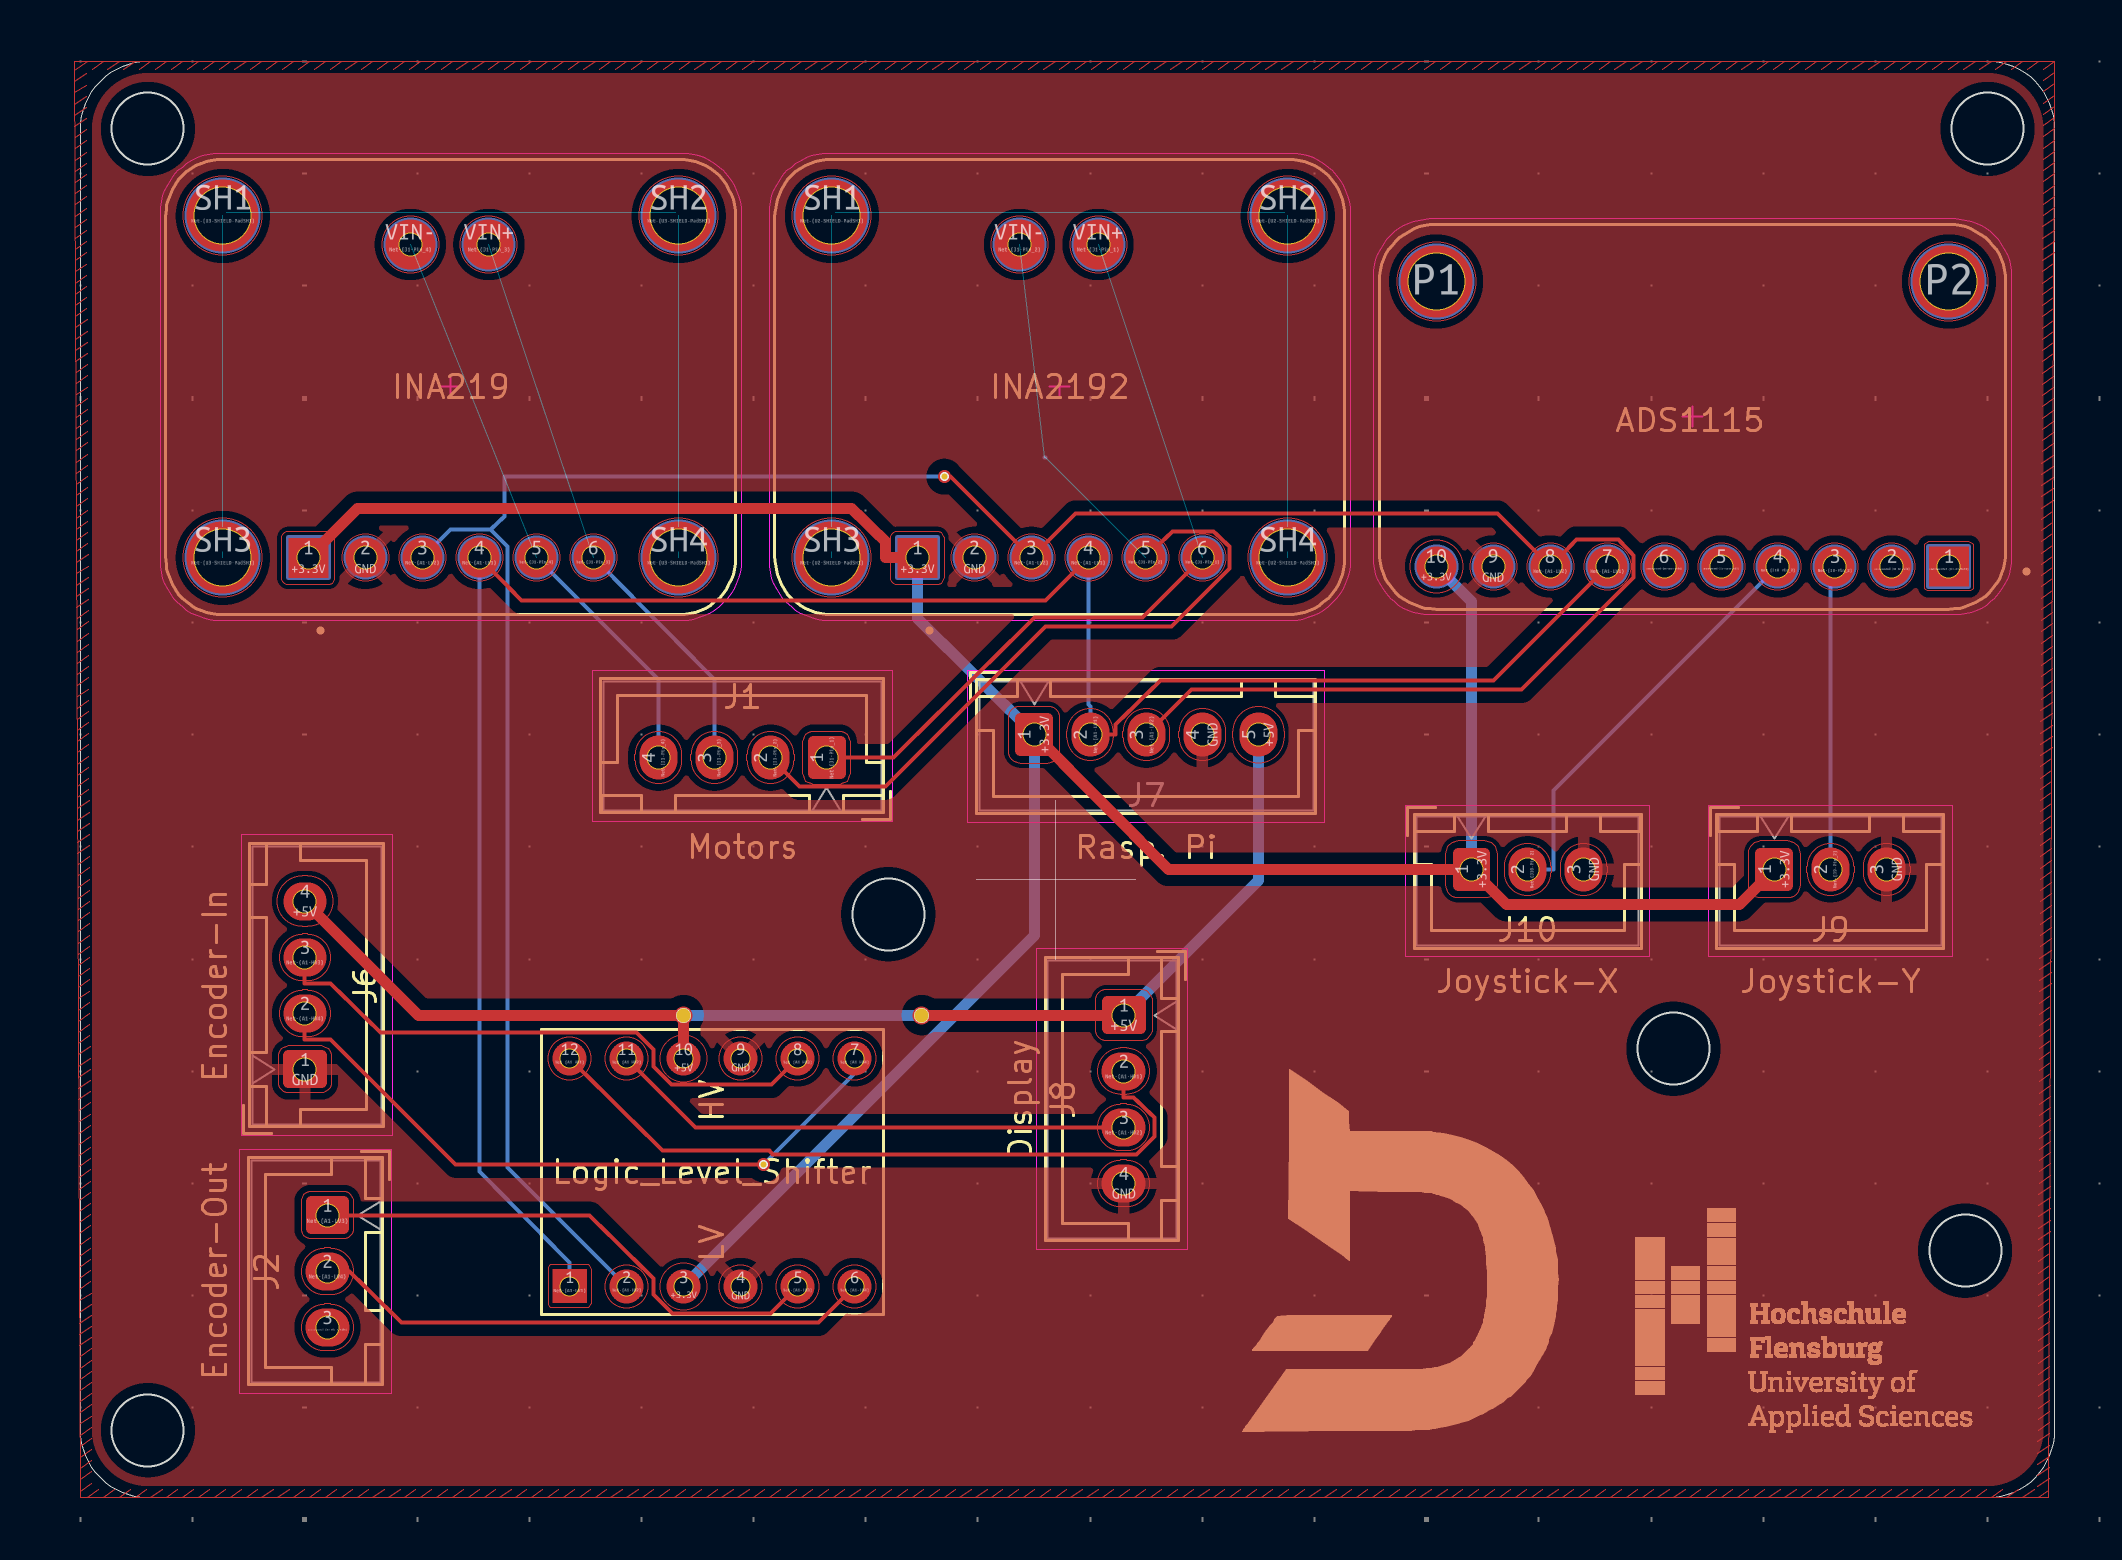
\includegraphics[width=\linewidth]{images/pcb_board2.png}
        \caption{PCB routing with modules, connectors, and power rails.}
    \end{subfigure}
    \caption[Assembled custom PCB]{The assembled RetroScope custom PCB (KiCad design, manufactured via JLCPCB),
    consolidating the joystick ADC, current-sense modules, level shifting, endstop/button
    connectors, and power rails. The board files are listed in Appendix~\ref{app:pcb}.}
    \label{fig:pcb}
\end{figure}

Table~\ref{tab:wiring} summarises the signal routing: the Sangaboard UART,
the level-shifted encoder inputs, the endstop and buttons, the shared I\textsuperscript{2}C bus with
its device addresses, and the power rails. The full pin map and the KiCad/Gerber references are
reproduced in Appendix~\ref{app:wiring} and Appendix~\ref{app:pcb}.

\begin{table}[H]
    \centering
    \caption[GPIO, I2C, UART, and power routing]{GPIO, I\textsuperscript{2}C, UART, and power routing of the prototype (BCM GPIO numbering).}
    \label{tab:wiring}
    \begin{tabular}{@{}L{3.4cm} L{4.3cm} L{6.0cm}@{}}
        \toprule
        \textbf{Subsystem} & \textbf{Pins / address} & \textbf{Notes} \\
        \midrule
        Sangaboard (UART) & GPIO 14 (TXD), 15 (RXD) & Full PL011 UART, Bluetooth disabled to free it \\
        Sangaboard control lines & GPIO 4, 8, 11, 23, 24, 25 & Stepper control / step signalling \\
        Rotary encoder & GPIO 17, 27 & Through 5\,V\ to 3.3\,V level shifter \\
        Endstop & GPIO 16 & Focus-axis (Z) safety limit \\
        Push buttons & GPIO 6, 13, 19, 26 & \\
        I\textsuperscript{2}C bus & GPIO 2 (SDA), 3 (SCL) & Shared by the modules below \\
        \quad ADS1115 & 0x48 & Joystick ADC \\
        \quad INA219 ($\times2$) & 0x40, 0x41 & Current-sense hardware \\
        \quad Touchscreen & 0x38, 0x45 & Touch controller and backlight \\
        Power rails & 5\,V, 3.3\,V, GND & Common ground \\
        \bottomrule
    \end{tabular}
\end{table}

\subsection{Software Layering: Drivers, Services, Domain Logic, and UI Bridges}

The software architecture is separated into layers. Drivers access hardware such as Sangaboard, joystick ADC, encoder, buttons, endstop, and camera sources. Services implement application behavior such as motion control, autofocus, focus stacking, tile scanning, image storage, updates, and REST API lifecycle. Domain modules implement pure calculations such as scan planning, focus metrics, focus blending, and calibration helpers. Bridge classes expose service state and commands to QML using Qt properties, signals, and slots. QML files implement the user interface.

This structure was explicitly motivated by maintainability and expandability.The QML views should not directly depend on low-level services or drivers. A new subsystem can be added by implementing a service or driver, exposing it through a bridge, and connecting it to QML. The design also supports unit testing because domain logic and services can be tested independently from the full UI. Figure~\ref{fig:software-layers} shows the resulting layering and the separate REST path.

The repository contains tests for calibration, autofocus, motion control, settings, gallery storage, tile scanning, REST API behavior, and camera helpers. These tests are not a substitute for physical measurement, but they provide evidence that the software behavior is intentionally structured and the components are testable in isolation.

\begin{figure}[H]
    \centering
    \begin{adjustbox}{max width=\linewidth}
    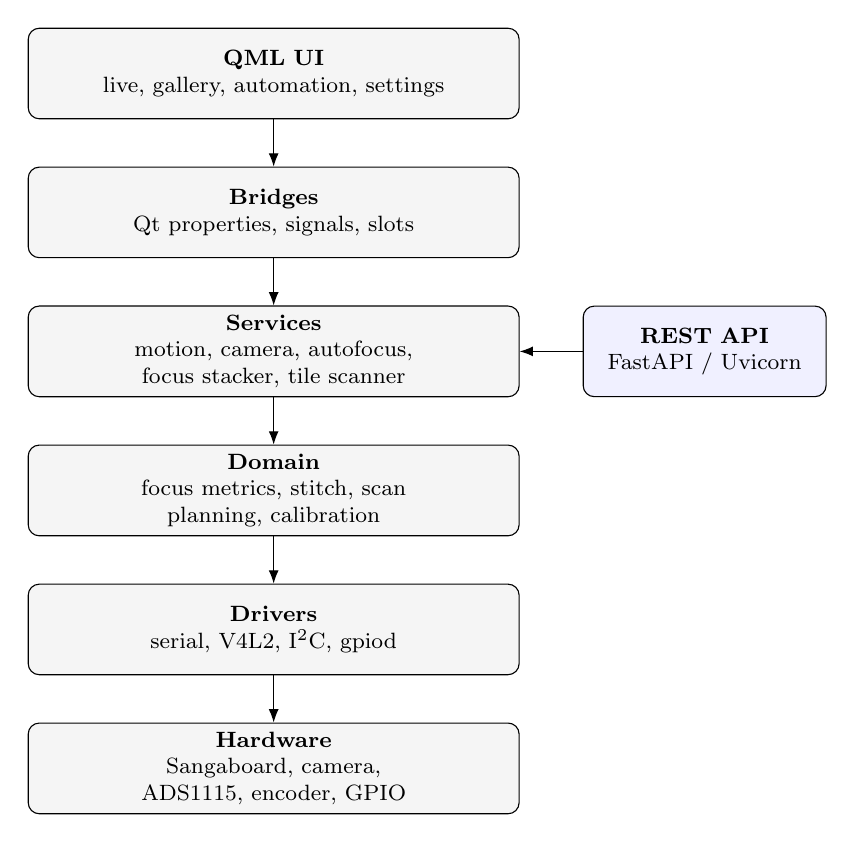
\begin{tikzpicture}[font=\footnotesize,
        box/.style={draw, rounded corners, align=center, minimum height=1.15cm,
                    text width=6.0cm, fill=gray!8},
        api/.style={box, text width=2.85cm, fill=blue!6},
        node distance=6mm]
        \node[box] (ui) {\textbf{QML UI}\\ live, gallery, automation, settings};
        \node[box, below=of ui] (br) {\textbf{Bridges}\\ Qt properties, signals, slots};
        \node[box, below=of br] (svc) {\textbf{Services}\\ motion, camera, autofocus, focus stacker, tile scanner};
        \node[api, right=8mm of svc] (api) {\textbf{REST API}\\ FastAPI / Uvicorn};
        \node[box, below=of svc] (dom) {\textbf{Domain}\\ focus metrics, stitch, scan planning, calibration};
        \node[box, below=of dom] (drv) {\textbf{Drivers}\\ serial, V4L2, I\textsuperscript{2}C, gpiod};
        \node[box, below=of drv] (hw) {\textbf{Hardware}\\ Sangaboard, camera, ADS1115, encoder, GPIO};

        \draw[-{Latex}] (ui)--(br);
        \draw[-{Latex}] (br)--(svc);
        \draw[-{Latex}] (api.west)--(svc.east);
        \draw[-{Latex}] (svc)--(dom);
        \draw[-{Latex}] (dom)--(drv);
        \draw[-{Latex}] (drv)--(hw);
    \end{tikzpicture}
    \end{adjustbox}
    \caption[Layered software architecture]{Layered software architecture. Hardware access is isolated in drivers. Services implement
    application behaviour. Domain modules hold pure calculations. Bridge classes expose
    state and commands to the QML touch interface and a FastAPI service offers remote access to the
    same services.}
    \label{fig:software-layers}
\end{figure}


\subsection{Camera Pipeline, Image Storage, and Metadata}

The camera service stores the latest analysis frame, emits histogram and focus-score updates, and provides full-resolution capture through a native recording backend. The frame-analysis path is used for live metrics and calibration support. The native capture path is used for snapshots, focus stacks, and tile scans when consistent full-resolution images are required. The gallery and image store manage thumbnails, metadata, and capture listing.

The project implements OME-TIFF. Focus stacks and tile scans can include multiple series, such as a blended or stitched result and the individual captured frames with coordinates. This makes the stored data more useful for external inspection and scientific workflows than one or more plain PNG images file would be.

\subsection{Configuration, Mock Mode, and Deployment}

Configuration is centralized in JSON-based config files. Objective profiles store magnification, numerical aperture, backlash values, pixel scale, depth-of-field steps, focus-stack step, and autofocus range. Other configuration groups cover UI state, capture root, API settings, input behavior, motor calibration, camera settings, objective detection, autofocus, and button mappings.

Mock mode allows desktop development without microscope hardware. It is important because the platform combines many hardware-dependent services. Without mock mode, testing UI changes, calibration flows, and gallery behavior would require the full physical microscope. Deployment on the Raspberry Pi includes additional setup steps for services and hardware configuration. A bash script included in the repository automates the installation of dependencies, configuration of services, and setup of the application to run on startup.


\newpage
\section{Motion Control and Backlash Compensation}\label{sec:motion}
\subsection{Motion-Control Pipeline}

\subsection{Manual Motion Through Touch UI, Joystick, and Encoder}

\subsection{Low-Cost Geared Stepper Behavior}

\subsection{Stage Scale and Axis Asymmetry}

\subsection{Software Backlash Compensation Model}

\subsection{Blocking Moves and Motion Diagnostics}

\subsection{Limits of Open-Loop Motion Control}


\newpage
\section{Calibration Process}\label{sec:calibration}
\subsection{Purpose of Calibration in the Retrofit Platform}

\subsection{Calibration Wizard Workflow}

\subsection{Objective Profiles and Pixel Scale Calibration}

\subsection{Scaling Calibration Across Objectives}

\subsection{Stage Scale Calibration for X and Y}

\subsection{Backlash Calibration}

\subsection{Focus, Depth-of-Field, and Autofocus Calibration}

\subsection{Soft Limits, Configuration Storage, and Reproducibility}

\subsection{Calibration Limitations}


\newpage
\section{Automated Microscopy Workflows}\label{sec:workflows}
\subsection{Calibrated Live View and Measurement}

\subsection{Autofocus}

\subsection{Focus Stacking}

\subsection{Tile Scanning and Stitching}

\subsection{Gallery, Metadata, and Data Export}

\subsection{Role of the Workflows in Validating the Platform}


\newpage
\section{Evaluation}\label{sec:evaluation}
\subsection{Evaluation Setup}

\subsection{Parametric Adapter Adaptability}

\subsection{Hardware Cost and Reproducibility}

\subsection{Motion Accuracy and Backlash Compensation}

\subsection{Calibration Consistency}

\subsection{Automated Workflow Reliability}

\subsection{REST API Functionality and Remote Access}

\subsection{Summary of Evaluation Results}


\newpage
\section{Discussion}
\subsection{Answering the Research Questions}

RQ1 asked whether a retrofit platform can add motorized control and digital imaging to vintage microscopes while remaining adaptable to different mechanical designs through parametric modelling. The prototype shows that this is feasible at the level of a working artifact. It adds motorized XY and Z movement, digital camera preview, calibration workflows, and automated capture workflows to the Nikon Optiphot 66 used during development. Adaptability is supported by the parametric Fusion model and by a mechanical strategy based on common microscope control interfaces, and it is demonstrated virtually. Editing the model parameters regenerates the adapter geometry for different body dimensions. Because only one suitable vintage instrument was available, this evidence is design-level rather than physical. The answer is therefore positive as a design principle, demonstrated virtually through parametric variation, while a broad empirical claim would still require adapting and building the platform on additional physical microscope bodies.

RQ2 asked whether a low-cost prototype can provide sufficiently consistent scale, motion, and positioning behavior for automated microscopy. The prototype demonstrates that low-cost open-loop hardware can be made usable, but only when its limitations are treated as part of the system design. The implemented system provides calibrated stage scales, separate X/Y/Z backlash values, soft limits, blocking movement for capture workflows, and a per-axis slack model for backlash behavior. The evaluation confirms that 4x stage-scale measurements are repeatable, especially for 200-step moves, and that hysteresis compensation substantially improves the X axis in the 200-step condition. However, without closed-loop position feedback, the system tracks commanded position rather than measured stage position. The evidence therefore supports practical consistency for prototype workflows, while precision claims must remain bounded by the measured variability and by the open-loop nature of the hardware.

RQ3 asked to what extent image-based calibration can enable automated workflows such as autofocus, focus stacking, and tile scanning. The implemented calibration system provides objective profiles, pixel scale, stage scale, backlash values, and derived scaling across objectives. These calibrated quantities allow the software to translate image observations and workflow settings into motor commands, overlap planning, focus ranges, and measurement units. In the workflow evaluation, autofocus, focus stacking, and tile scanning each completed 10/10 runs for the 4x, 20x, 40x, and 63x profiles. The answer is that image-based calibration is a necessary layer for these workflows, but reliability also depends on motion compensation, blocking logic, and careful performance management.

\subsection{Trade-Offs of the Retrofit Approach}

The main advantage of retrofitting is reuse. A vintage microscope can gain digital imaging and automation without replacing the optical instrument. The platform can remain affordable, inspectable, and adaptable. It can also be built around open-source artifacts, which supports modification and learning.

The main disadvantage is inherited uncertainty. The retrofit must work through existing controls, printed adapters, and low-cost motors. The software does not control a precision stage directly. It controls a chain of mechanics that includes slack, friction, flex, and calibration uncertainty. This makes the system more sensitive to physical assembly and calibration than an integrated commercial platform.

This trade-off is acceptable for the stated goal of the thesis. RetroScope is not presented as a replacement for high-end motorized microscopes. It is presented as an open platform that extends older microscopes lifetime with useful digital and automated capabilities.

\subsection{Low-Cost Hardware Versus Precision}

Low-cost hardware expands accessibility but reduces precision margins. The 28BYJ motors, printed gears, and open-loop control are affordable and easy to reproduce, but they create backlash and motion variability. The Raspberry Pi provides enough computation for the application, but performance-sensitive paths such as frame analysis and gallery rendering had to be optimized.

The prototype shows that these limitations can be managed, but not ignored. The final system separates live preview from frame analysis, uses native capture for high-resolution imaging, adds blocking moves for capture workflows, and tracks backlash slack. These changes are all consequences of using constrained hardware.

\subsection{Software Compensation Versus Mechanical Limits}

Software compensation is powerful when the mechanical error is predictable. Backlash is partly predictable because direction changes consume slack before physical movement occurs. The hysteresis-band model captures this deterministic behavior better than treating backlash as random noise. Similarly, stage-scale calibration can correct systematic differences between X and Y movement.

Software compensation is less effective when the mechanical state changes unpredictably. Printed parts can flex, screws can loosen, the stage can be moved by hand, friction can change after lubrication, and a motor can miss steps. Without direct feedback, the software cannot observe all of these events. This is why the platform invalidates backlash history after certain events and why calibration remains central.

The practical lesson is that mechanical and software design must be co-developed. The adapter should reduce backlash and flex as much as possible, while the software compensates what remains. Neither side is sufficient alone.

\subsection{Limitations}

The main limitation is that the prototype has been built and evaluated on a single physical microscope body, the Nikon Optiphot 66, because no second suitable vintage instrument was available and a second physical build was out of scope. This limits empirical claims about general mechanical adaptability. The parametric model supports adaptation and this is demonstrated virtually through parameter variation, but a stronger evaluation would build the platform on additional physical microscopes with different focus and stage geometries.

A second limitation is the lack of closed-loop position feedback. The platform tracks commanded motor position, not measured sample position. This affects motion accuracy, backlash compensation, and repeatability. The system can be useful without encoders, but accuracy claims must remain bounded by the open-loop nature of the design.

A third limitation is the scope of the quantitative evaluation data. The current datasets cover 4x stage-scale, 4x motion behavior, 4x calibration repeatability, and workflow reliability for 4x, 20x, 40x, and 63x. They do not include other objective profiles, closed-loop position measurements, or physical validation on a second microscope body.

Finally, the thesis is partly based on a evolving software artifact. This creates a risk that described behavior may drift from the final repository state. The evaluation was run on a specific commit: 13ada32.


\newpage
\section{Conclusion and Future Work}
\subsection{Summary}

This thesis presented RetroScope, an open retrofit platform for motorizing and digitizing vintage microscopes. The work started from the observation that many microscopes share user-facing control interfaces such as focus knobs, and XY-stage knobs. RetroScope uses these interfaces instead of replacing the microscope's internal mechanics. A parametric mechanical adapter, low-cost embedded electronics, modular software stack, and image-based calibration process are combined into a working prototype.

The prototype demonstrates motorized XY and Z control, live digital imaging, objective profiles, calibrated measurement, autofocus, focus stacking, tile scanning, and REST-based remote access. The workflows are enabled by calibration and motion compensation rather than by high-end mechanical hardware. This is the central result of the thesis: a low-cost retrofit can become useful when mechanical adaptation, embedded control, software architecture, and calibration are designed together.

\subsection{Future Work}

Future work should begin with extending the quantitative validation. The current evaluation already covers 4x stage scale, 4x motion accuracy, 4x calibration repeatability, and workflow reliability across several objective profiles. The next step is to add higher-magnification calibration, motion, and stage-scale datasets, objective quality metrics for focus stacks and tile scans, and a comparison of alternative higher-performance, higher-cost component choices. The parametric adapter's adaptability is demonstrated virtually in this thesis through parameter variation on the Nikon Optiphot 66 model. Building the platform on additional physical microscope bodies would turn this into empirical evidence and further strengthen the adaptability claim.

The mechanical design could be improved through stiffer materials, metal inserts or machined parts in high-load areas, and better gear support. The motion system could be improved through closed-loop feedback, for example with motor encoders, stage encoders, optical tracking, or other position sensors.

The software could be extended with richer REST endpoints, remote live-view streaming, additional capture formats, and more robust stitching.

RetroScope therefore remains both a working prototype and a platform for further development. Its main value is not that it removes all limitations of low-cost retrofit hardware, but that it shows a coherent path for giving vintage microscopes a longer lifetime with programmable and digital capabilities.


% ---------- APPENDIX
\newpage
\appendix
\section{Appendix}
\subsection{Bill of Materials and Cost Breakdown}
\subsection{Custom PCB Schematic and Gerber Reference}
\subsection{GPIO, I2C, UART, and Power Wiring}
\subsection{Parametric Fusion Model Parameters}
\subsection{3D-Printing and Assembly Notes}
\subsection{Calibration Protocol}
\subsection{Backlash and Stage-Scale Measurement Data}
\subsection{REST API Endpoint Reference}
\subsection{Configuration Examples}
\subsection{Test Protocols and Raw Evaluation Data}
\subsection{User Interface Screenshots}
\subsection{Installation and Deployment Guide}
\subsection{List of Released Open-Source Artifacts}
\subsection{Declaration: Use of Generative AI}
\subsection{Declaration on Examinations}


\newpage
\phantomsection
\addcontentsline{toc}{section}{Glossary}
\glsaddall
\printglossary[title={Glossary}, toctitle={Glossary}, nonumberlist]

\newpage
\section*{List of Abbreviations}
\addcontentsline{toc}{section}{List of Abbreviations}
\addcontentsline{toc}{subsection}{Glossary}
\subsection*{Acronyms}

\begin{acronym}
    \acro{DS}{Data Science}
    \acro{DM}{Data Mining}
    \acro{ML}{Machine Learning}
    \acro{EO}{Executive Order}
    \acro{AI}{Artificial Intelligence}
    \acro{NLP}{Natural Language Processing}
\end{acronym}

\newpage
\section*{List of Figures}
\addcontentsline{toc}{section}{List of Figures}
\renewcommand{\listfigurename}{}  % suppresses title
\listoffigures

\newpage
\section*{List of Tables}
\addcontentsline{toc}{section}{List of Tables}
\renewcommand{\listtablename}{}   % suppresses title
\listoftables
%\input{codeAvailability} %TODO

\newpage
%\addcontentsline{toc}{subsection}{Literaturverzeichnis}
% \nocite{*}

\printbibliography[title=References, heading=bibintoc]

\clearpage
\phantomsection
\addcontentsline{toc}{section}{Declaration: Use of Generative AI}
\section*{Declaration: Use of Generative AI}

The following generative AI tools were used in this thesis:

\begin{itemize}
  \item GitHub Copilot in VS Code was used for inline code-completion suggestions during implementation and writing.
  \item ChatGPT (OpenAI) \& Claude (Anthropic) used to support brainstorming, quick research, and the generation of selected parts of the code (e.g. unit tests). AI-assisted scripts and functions are marked in the source code via comments.
  \item DeepL write (DeepL SE) were used in language editing and grammatical proof-reading.
\end{itemize}

All AI-generated material was critically reviewed, edited, and verified by the author. No generative AI system was used to produce original scientific results, experimental data, proofs, or final implementations of algorithms. The author assumes full responsibility for the content, correctness, and originality of this thesis.

\clearpage
\phantomsection
\addcontentsline{toc}{section}{Declaration on examinations}
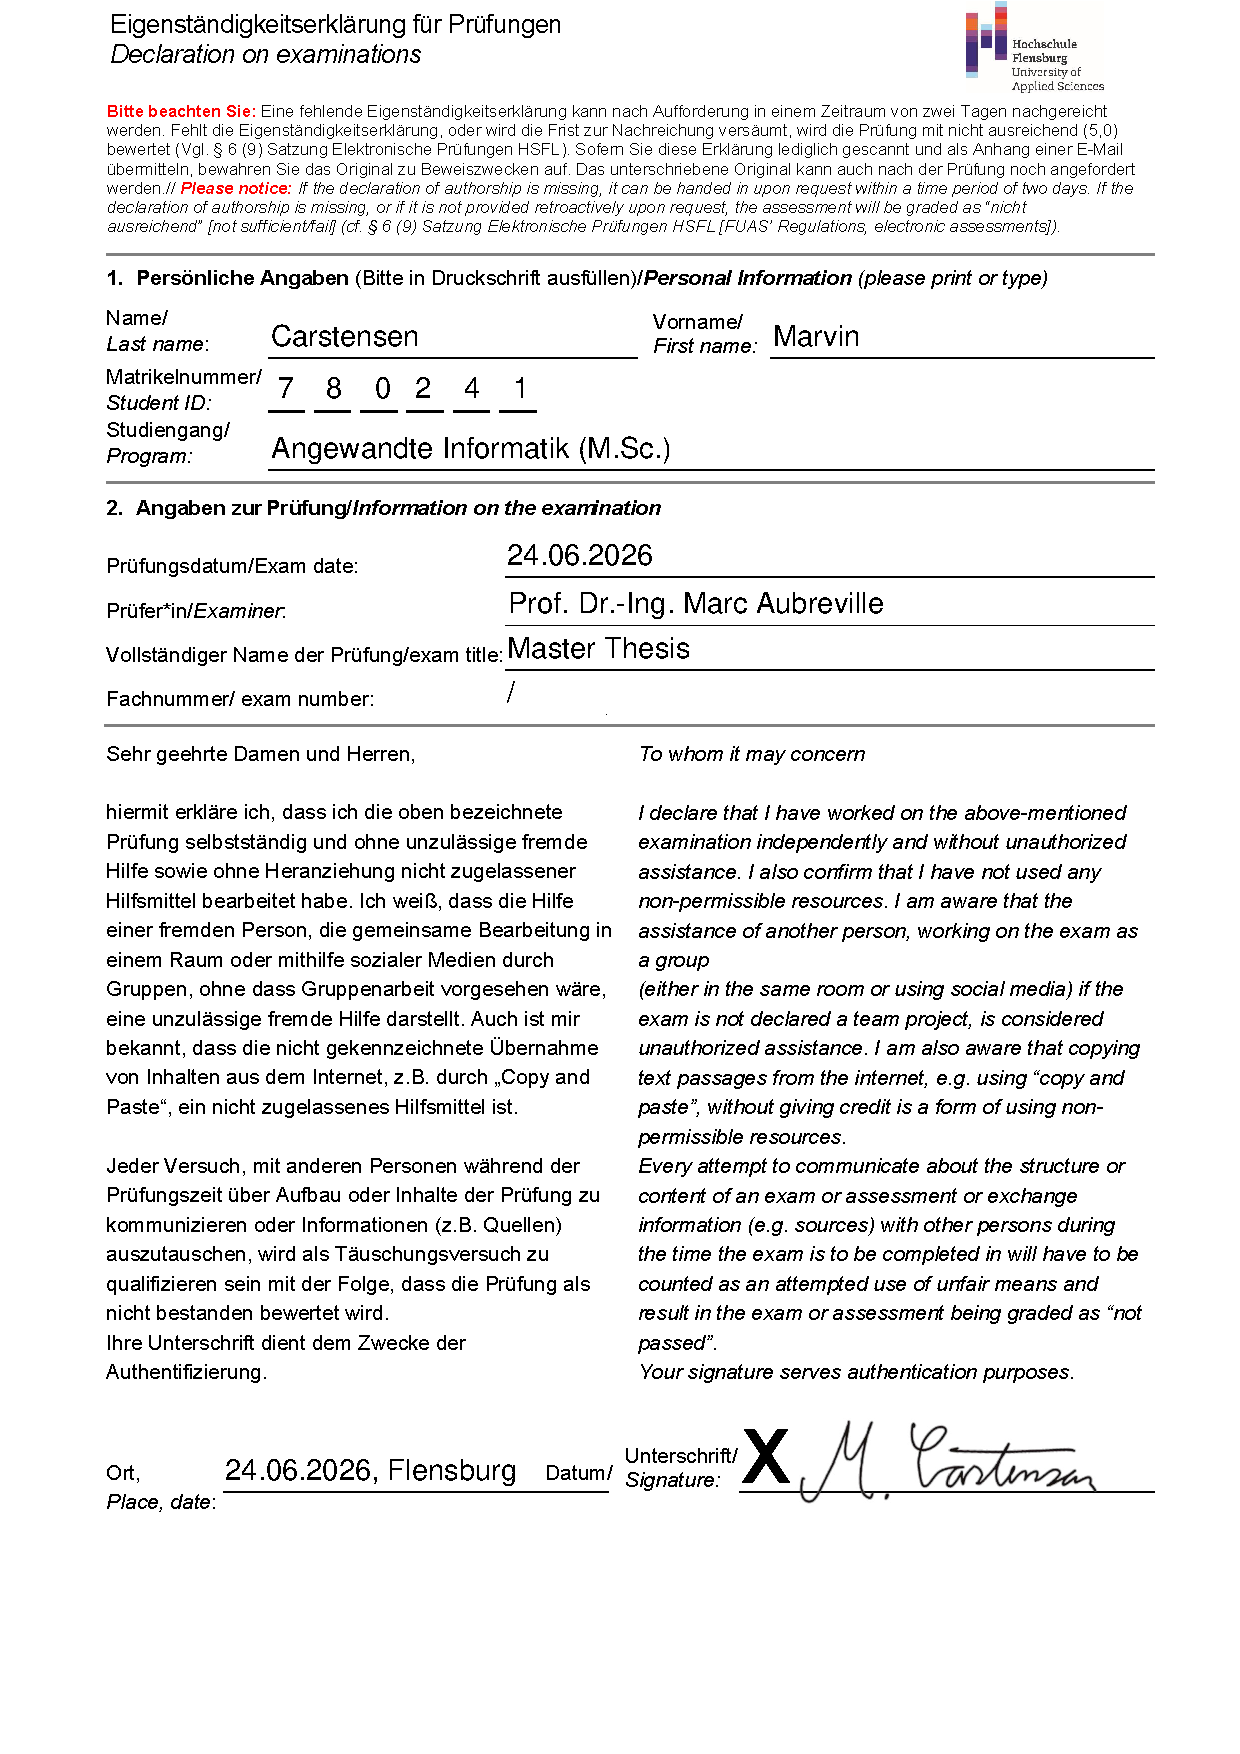
\includepdf[
    pages=-,
    pagecommand={},
    offset=0 -1cm
]{Eigenstandigkeitserklarung_zur_prufung_NEU_flattened.pdf}

\end{document}
